\documentclass[a4paper]{scrreprt}
\usepackage[german]{babel}
\usepackage[utf8]{inputenc}
\usepackage[T1]{fontenc}
\usepackage{graphicx}
\usepackage{float}
\graphicspath{ {images/} }
\usepackage{ae}

\begin{document}
    \chapter{Anwendungsfälle}
    		\begin{figure}[H]
			\centering
			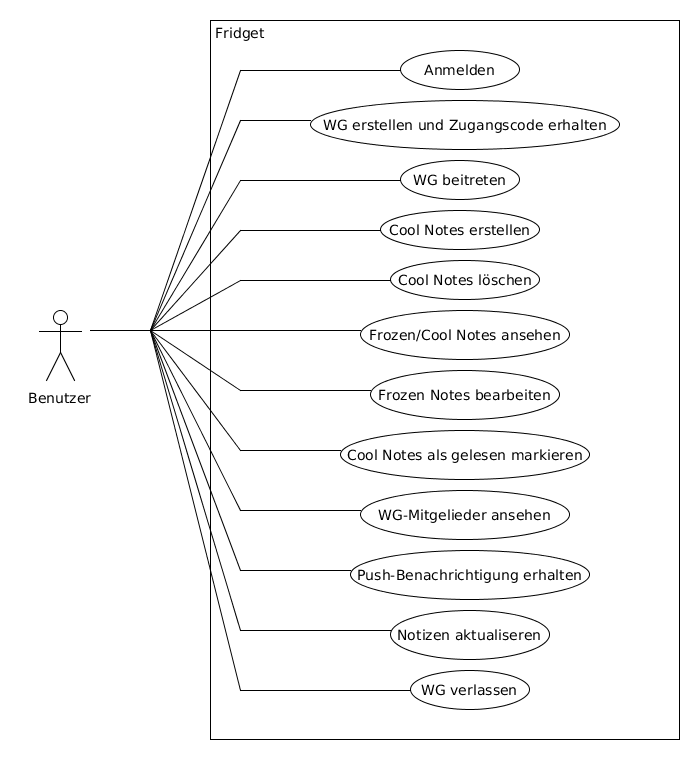
\includegraphics[scale = .6]{anwendungsfalldiagramm.png}
			\caption{Anwendungsfalldiagramm}
		\end{figure}
    		    		
        \section{Anmelden}
        \textbf{Teilnehmende Akteure}: Benutzer \\
		\textbf{Eingangsbedingungen}: Der Benutzer hat Fridget installiert und besitzt ein Google-Account. Das Internet ist verfügbar. \\
		\textbf{Ausgangsbedingung}: Der Benutzer hat sich angemeldet. \\
		\textbf{Ereignisfluss}: Benutzer meldet sich mit Google-Account an
		
		\section{WG erstellen und Zugangscode erhalten}
		\textbf{Teilnehmende Akteure}: Benutzer \\
		\textbf{Eingangsbedingungen}: Der Benutzer hat sich angemeldet. Das Internet ist verfügbar. \\
		\textbf{Ausgangsbedingung}: Eine WG wurde erstellt und ein Zugangscode wurde in der App angezeigt. \\
		\textbf{Ereignisfluss}: Benutzer wählt WG erstellen aus $\rightarrow$ Benutzer gibt einen WG-Namen ein $\rightarrow$ Benutzer bestätigt das Erstellen $\rightarrow$ WG wird erstellt $\rightarrow$ Zugangscode wird generiert
		
		\section{WG beitreten}
		\textbf{Teilnehmende Akteure}: Benutzer \\
		\textbf{Eingangsbedingungen}: Der Benutzer hat sich angemeldet und besitzt einen gültigen Zugangscode. Die WG ist nicht voll. Das Internet ist verfügbar. \\
		\textbf{Ausgangsbedingung}: Der Benutzer ist einer WG beigetreten. \\
		\textbf{Ereignisfluss}: Benutzer wählt Zugangscode eingeben aus $\rightarrow$ Benutzer gibt den Zugangscode ein $\rightarrow$ Benutzer bestätigt das Eingeben
		
		\section{Cool Notes erstellen}
		\textbf{Teilnehmende Akteure}: Benutzer \\
		\textbf{Eingangsbedingungen}: Der Benutzer hat sich angemeldet und ist einer WG beigetreten. Die Pinnwand ist nicht voll. Das Internet ist verfügbar. \\
		\textbf{Ausgangsbedingung}: Eine Cool Note wurde erstellt und mit zugehörigen Magnet auf der Pinnwand angezeigt. \\
		\textbf{Ereignisfluss}: Benutzer tippt auf den Plus-Button $\rightarrow$ Benutzer gibt die Überschrift mit oder ohne dem Textinhalt ein $\rightarrow$ Benutzer bestätigt das Erstellen
		
		\section{Cool Notes löschen}
		\textbf{Teilnehmende Akteure}: Benutzer \\
		\textbf{Eingangsbedingungen}: Der Benutzer hat die Großansicht einer Cool Note, die nicht von ihm erstellt wurde, geöffnet. Das Internet ist verfügbar. \\
		\textbf{Ausgangsbedingung}: Die Cool Note wurde gelöscht. \\
		\textbf{Ereignisfluss}: Benutzer tippt auf den Minus-Button $\rightarrow$ Benutzer bestätigt das Löschen
		
		\section{Frozen/Cool Notes ansehen}
		\textbf{Teilnehmende Akteure}: Benutzer \\
		\textbf{Eingangsbedingungen}: Der Benutzer hat sich angemeldet und ist einer WG beigetreten. Die Pinnwand ist nicht leer. Das Internet ist verfügbar. \\
		\textbf{Ausgangsbedingung}: Großansicht einer Frozen/Cool Note wurde angezeigt. \\
		\textbf{Ereignisfluss}: Benutzer tippt auf eine Frozen/Cool Note an
		
		\section{Frozen Notes bearbeiten}
		\textbf{Teilnehmende Akteure}: Benutzer \\
		\textbf{Eingangsbedingungen}: Der Benutzer hat die Großansicht einer Frozen Note geöffnet. Das Internet ist verfügbar. \\
		\textbf{Ausgangsbedingung}: Eine Frozen Note wurde bearbeitet. \\
		\textbf{Ereignisfluss}: Benutzer tippt auf den Edit-Button $\rightarrow$ Benutzer bearbeitet die Frozen Note $\rightarrow$ Benutzer bestätigt das Bearbeiten
		
		\section{Cool Notes als gelesen markieren}
		\textbf{Teilnehmende Akteure}: Benutzer \\
		\textbf{Eingangsbedingungen}: Der Benutzer hat die Großansicht einer Cool Note, die nicht von ihm erstellt wurde, geöffnet. Die Cool Note wurde noch nicht als gelesen markiert. Das Internet ist verfügbar. \\
		\textbf{Ausgangsbedingung}: Eine Cool Note wurde für einen Benutzer als gelesen markiert. \\
		\textbf{Ereignisfluss}: Benutzer markiert die Checkbox als gelesen
		
		\section{WG-Mitgelieder ansehen}
		\textbf{Teilnehmende Akteure}: Benutzer \\
		\textbf{Eingangsbedingungen}: Der Benutzer hat sich angemeldet und ist einer WG beigetreten. Das Internet ist verfügbar. \\
		\textbf{Ausgangsbedingung}: Die aktuellen WG-Mitglieder mit zugehörigem Magnet wurden angezeigt. \\
     	\textbf{Ereignisfluss}: Benutzer öffnet die App-Menü $\rightarrow$ Benutzer wählt WG-Mitgelieder ansehen aus
		
		\section{Push-Benachrichtigung erhalten}
		\textbf{Teilnehmende Akteure}: Benutzer \\
		\textbf{Eingangsbedingungen}: Der Benutzer hat sich angemeldet und ist einer WG beigetreten. Der Benutzer hat ``Push-Benachrichtigung'' von Fridget aktiviert. Das Internet ist verfügbar. \\
		\textbf{Ausgangsbedingung}: Die Push-Benachrichtigung wurde auf den Geräten des Benutzers angezeigt. \\
		\textbf{Ereignisfluss}: Eine neue Cool Note wird erstellt $\rightarrow$ Push-Benachrichtigung wird generiert und abgeschickt
		
		\section{Notizen aktualisieren}
		\textbf{Teilnehmende Akteure}: Benutzer \\
		\textbf{Eingangsbedingungen}: Der Benutzer hat sich angemeldet und ist einer WG beigetreten. Das Internet ist verfügbar. \\
		\textbf{Ausgangsbedingung}: Die Änderungen von Notizen wurden mit dem Server synchronisiert. \\
		\textbf{Ereignisfluss}: Benutzer swipt die Pinnwand hinunter $\rightarrow$ Notizen werden aktualisiert
		
		\section{WG verlassen}
		\textbf{Teilnehmende Akteure}: Benutzer \\
		\textbf{Eingangsbedingungen}: Der Benutzer hat sich angemeldet und ist einer WG beigetreten. Das Internet ist verfügbar. \\
		\textbf{Ausgangsbedingung}: Der Benutzer hat die WG verlassen. \\
		\textbf{Ereignisfluss}: Benutzer öffnet die App-Menü $\rightarrow$ Benutzer wählt die WG verlassen aus $\rightarrow$ Benutzer bestätigt das Verlassen
\end{document}